%----------------------------------------------------------------------------------------
%	PACKAGES AND DOCUMENT CONFIGURATIONS
%----------------------------------------------------------------------------------------

\documentclass{article}

\usepackage{siunitx} % Provides the \SI{}{} and \si{} command for typesetting SI units
\usepackage{graphicx} % Required for the inclusion of images
\usepackage{natbib} % Required to change bibliography style to APA
\usepackage{amsmath} % Required for some math elements 
\setlength\parindent{12pt} % Removes all indentation from paragraphs
%\usepackage{times} % Uncomment to use the Times New Roman font

\usepackage[export]{adjustbox}

\usepackage[utf8]{inputenc} % Język polski
\usepackage{polski}
\usepackage[polish]{babel}

\usepackage[top=1in, bottom=1.25in, left=1.25in, right=1.25in]{geometry} % Marginesy
\usepackage{listings} % Kod programu
\usepackage{indentfirst} % Wcięcie przy pomocy \par
\usepackage{multicol} % Kilka kolumn dla itemize
\usepackage{color} % Kolorowanie tekstu

%\renewcommand{\labelenumi}{\alph{enumi}.} % Zamienia litery w enumerate na a, b, c, ...
%----------------------------------------------------------------------------------------
%	DOCUMENT INFORMATION
%----------------------------------------------------------------------------------------

\title{Inżynieria Oprogramowania} % Title

\author{Jan \textsc{Pajdak} \\ Jakub \textsc{Majorek} \\ Sebastian \textsc{Łągiewski}} % Author name

\date{26.10.2017} % Date for the report
%\date{\today} % Date for the report

\begin{document}
	
	\maketitle % Insert the title, author and date
	
	%\begin{center}
	%\begin{tabular}{l r}
	%Data: & Semestr letni, 2017 \\ % Date the experiment was performed
	%Prowadzący: & Mgr inż. Tomasz Serafin% Instructor/supervisor
	%\end{tabular}
	%\end{center}
	
	\tableofcontents
	
	% If you wish to include an abstract, uncomment the lines below
	% \begin{abstract}
	% Abstract text
	% \end{abstract}
	
	%----------------------------------------------------------------------------------------
	%	SECTION 0
	%----------------------------------------------------------------------------------------
	
	%\newpage
	%\section{Tytuł}} 
	%\subsection{Tytuł}
	%\par Tekst
	
	%\begin{itemize}
	%	\item\textit{Tekst} - Opis
	%\end{itemize}
	
	%\begin{enumerate}
	%	\item Opis
	%\end{enumerate}
	
	%\begin{center}
	%	\includegraphics[scale=0.6, center]{nazwa_pliku}
	%\end{center}
	
	%\begin{lstlisting}[basicstyle=\small]
	%	kod programu;
	%\end{lstlisting}
	
	%----------------------------------------------------------------------------------------
	%	SECTION 1
	%----------------------------------------------------------------------------------------
	\newpage
	\section{Opis świata rzeczywistego}
	\subsection{Opis biznesowy}
	\subsubsection{Opis zasobów ludzkich}
	\par Aplikacja tworzona jest dla małego kina w którym z poziomu jednego komputera można zarządzać całym kinem - biblioteką filmów, seansami oraz rezerwacjami i sprzedażą biletów. Po uruchomieniu programu użytkownik musi zalogować się w systemie by uzyskać odpowiednie uprawnienia. Są dwa rodzaje uprawnień:
	\begin{enumerate}
		\item Menadżer - pełne uprawnienia
		\item Kasjer - tylko rezerwacje i sprzedaż biletów
	\end{enumerate}
	
	\par Menadżer może dodawać do katalogu filmów nowe pozycje. Katalog zawiera następujące informacje:
	\begin{multicols}{2}
		\begin{itemize}
			\item Tytuł filmu
			\item Reżyser
			\item Aktorzy
			\item Język
			\item Gatunek
			\item Długość
			\item Data premiery
			\item Sugerowany wiek widza
		\end{itemize}
	\end{multicols}
	
	\par Kolejnym zadaniem menadżera jest planowanie seansów. System przechowuje następujące informacje o seansach:
	\begin{multicols}{2}
		\begin{itemize}
			\item Numer sali
			\item Godzina
			\item Data
			\item Czas seansu
		\end{itemize}
	\end{multicols}
	
	\par Ostatnią funkcją jest zarządzanie sprzedażą - rezerwacje i sprzedaż biletów. Rezerwacja zawiera:
	\begin{multicols}{2}
		\begin{itemize}
			\item Seans
			\item Miejsce
			\item Data
			\item Dane klienta
		\end{itemize}
	\end{multicols}
	
	\subsubsection{Wymagania funkcjonalne}
	\par Dwa rodzaje uprawnień – menadżer: pełny dostęp do funkcjonalności programu; kasjer: dokonywanie rezerwacji i sprzedaż biletów.
	\par \textbf{Menadżer:}
	\begin{itemize}
		\item Dokonuje zakupów licencji na różne filmy
		\item Ustala ceny biletów
		\item Dodaje/modyfikuje/usuwa dane pozyskanych filmów.
		\item Planuje seanse
	\end{itemize}
	\par \textbf{Kasjer:}
	\begin{itemize}
		\item Dokonuje rezerwacji oraz ma wgląd do historii rezerwacji, gdzie może je modyfikować/usuwać
		\item Sprzedaje i drukuje bilety
	\end{itemize}
	
	\subsection{Uproszczony diagram}
	\begin{center}
		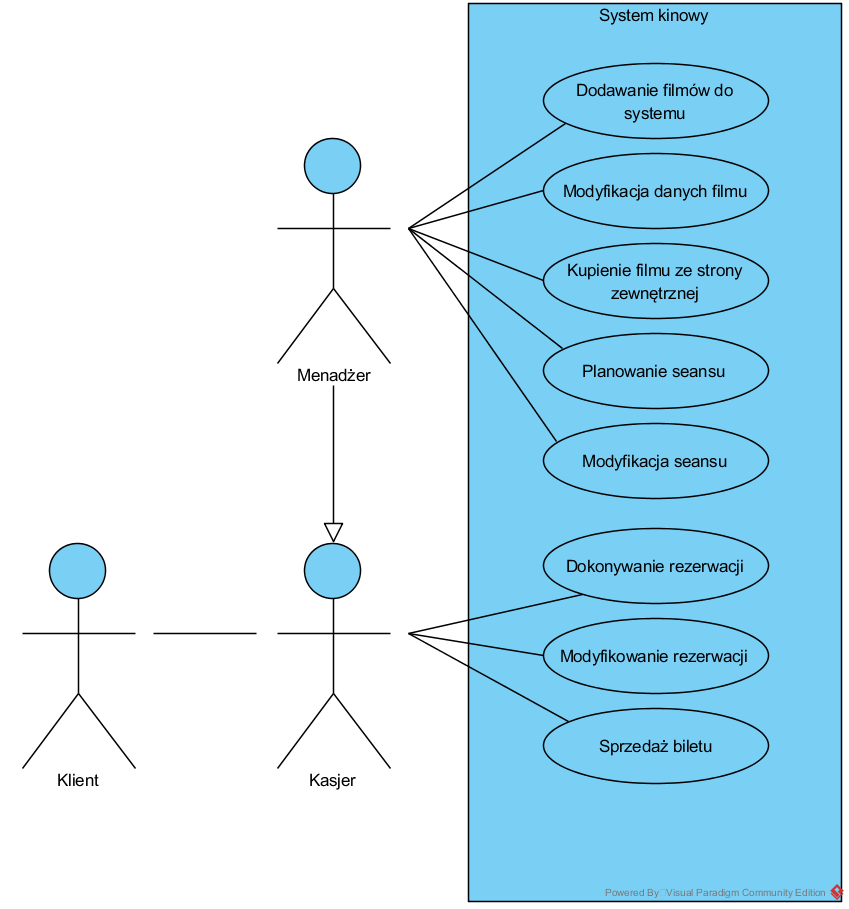
\includegraphics[scale=0.8, center]{UC-1}
	\end{center}
	
	%----------------------------------------------------------------------------------------
	%	SECTION 2
	%----------------------------------------------------------------------------------------
	\newpage
	\section{Przypadki użycia}
	
	\subsection{Diagram przypadków użycia}
	\begin{center}
		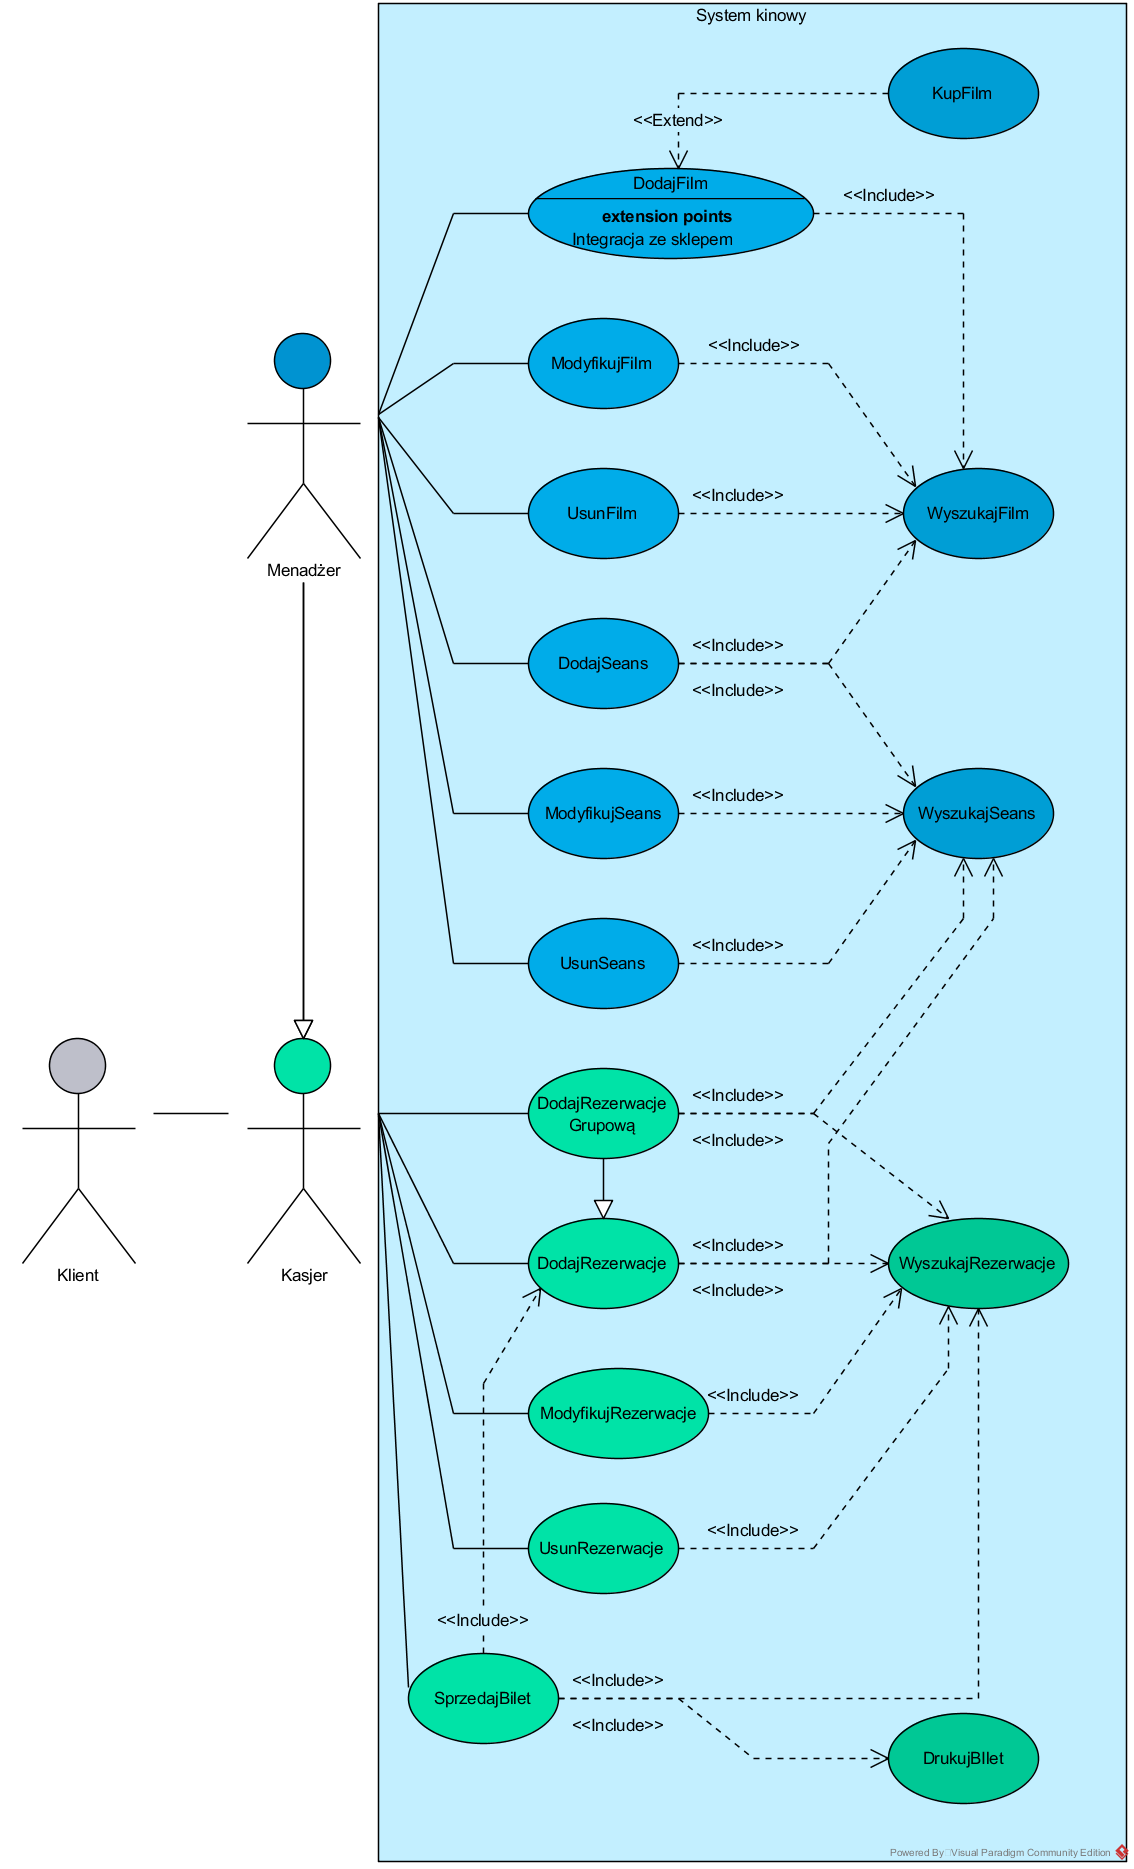
\includegraphics[scale=0.8, center]{UC-2}
	\end{center}
	\par Program zawiera dwa możliwe punkty rozszerzenia:
	\begin{enumerate}
		\item \textbf{BuyMovie} - integracja programu z serwisem sprzedającym filmy.
		\item \textbf{AddReservationGrupowa} - szybką rezerwacje kilku miejsc na raz.
	\end{enumerate}
	
	\newpage
	\subsection{Opis aktorów}
	\subsubsection{Menadżer}
	\par Menadżer ma dostęp do pełnej funkcjonalności programu - może w pełni zarządzać całym kinem.
	\par Przypadki użycia:
	\begin{itemize}
		\item \textbf{PU AddMovie} powiązane przez \textit{extend} z \textit{\textbf{PU BuyMovie}} oraz przez \textit{<<include>>} z \textit{\textbf{PU FindMovie}}
		\item \textbf{PU ModifyMovie} powiązane przez \textit{<<include>>} z \textit{\textbf{PU DeleteMovie}} i \textit{\textbf{PU FindMovie}}
		\item \textbf{PU AddShow} powiązane przez \textit{<<include>>} z \textit{\textbf{PU FindMovie}} i \textit{\textbf{PU FindShow}}
		\item \textbf{PU ModifyShow} powiązane przez \textit{<<include>>} z \textit{\textbf{PU DeleteShow}} i \textit{\textbf{PU FindShow}}
		\item \textbf{PU AddReservation} powiązane przez \textit{extend} z \textit{\textbf{PU AddReservationGrupowa}} oraz przez \textit{<<include>>} z \textit{\textbf{PU FindReservation}} i \textit{\textbf{PU FindShow}}
		\item \textbf{PU ModifyReservation} powiązane przez \textit{<<include>>} z \textit{\textbf{PU DeleteReservation}} i \textit{\textbf{PU FindReservation}}
		\item \textbf{PU SellTicket} powiązane przez \textit{<<include>>} z \textit{\textbf{PU FindReservation}} i \textit{\textbf{PU PrintTicket}}
	\end{itemize}
	
	\subsubsection{Kasjer}
	\par Kasjer może wyłącznie zarządzać rezerwacjami i sprzedawać bilety.
	\par Przypadki użycia:
	\begin{itemize}
		\item \textbf{PU AddReservation} powiązane przez \textit{extend} z \textit{\textbf{PU AddReservationGrupowa}} oraz przez \textit{<<include>>} z \textit{\textbf{PU FindReservation}} i \textit{\textbf{PU FindShow}}
		\item \textbf{PU ModifyReservation} powiązane przez \textit{<<include>>} z \textit{\textbf{PU DeleteReservation}} i \textit{\textbf{PU FindReservation}}
		\item \textbf{PU SellTicket} powiązane przez \textit{<<include>>} z \textit{\textbf{PU FindReservation}} i \textit{\textbf{PU PrintTicket}}
	\end{itemize}
	
	\subsubsection{Klient}
	\par Klient może dokonywać rezerwacji przez kasjera i kupować u niego bilety.
	
	\newpage
	\subsection{Zarządzanie katalogiem filmów}
	\subsubsection{PU AddMovie}
	\noindent \textbf{Opis}
	\newline \textbf{Cel: } Dodanie nowego filmu
	\newline \textbf{WS: } Brak
	\newline \textbf{WK: } Dodanie filmu o podanych atrybutach: Tytuł, gatunek, reżyser, aktorzy, długość, data premiery, język, sugerowany wiek widza
	\newline \textbf{Przebieg: }
	\begin{enumerate}
		\item Należy podać atrybuty filmu
		\item Należy wywołać \textit{\textbf{PU FindMovie}}, sprawdzić czy w bazie nie istnieje film o identycznych atrybutach. Jeżeli obecnie wprowadzany film nie jest duplikatem, dodajemy go do bazy.
	\end{enumerate}
	
	\subsubsection{PU BuyMovie}
	\noindent \textbf{Opis}
	\newline \textbf{Cel: } Dodanie nowego filmu przy użyciu integracji ze sklepem
	\newline \textbf{WS: } Brak
	\newline \textbf{WK: } Kupno filmu
	\newline \textbf{Przebieg: }
	\begin{enumerate}
		\item Należy wybrać i kupić film
		\item Należy wywołać \textit{\textbf{PU FindMovie}}, sprawdzić czy w bazie nie istnieje film o identycznych atrybutach. Jeżeli obecnie wprowadzany film nie jest duplikatem, dodajemy go do bazy.
	\end{enumerate}
	
	\subsubsection{PU ModifyMovie}
	\noindent \textbf{Opis}
	\newline \textbf{Cel: } Modyfikacja danego filmu
	\newline \textbf{WS: } Brak
	\newline \textbf{WK: } Podanie filmu o danym identyfikatorze
	\newline \textbf{Przebieg: }
	\begin{enumerate}
		\item Podanie ID seansu
		\item Należy wywołać \textit{\textbf{PU FindMovie}}, sprawdzić czy film o podanym ID istnieje. Jeśli istnieje, można zmodyfikować dany film lub wywołać \textit{\textbf{PU DeleteMovie}} w celu usunięcia filmu, w przeciwnym wypadku należy zakończyć PU.
	\end{enumerate}
	
	\subsubsection{PU DeleteMovie}
	\noindent \textbf{Opis }
	\newline \textbf{Cel:} Usunięcie filmu z BD
	\newline \textbf{WS: } Jest wywoływany z \textit{\textbf{PU ModifyMovie}}, jeśli dany film zostanie znaleziony za pomocą \textit{\textbf{PU FindMovie}}
	\newline \textbf{WK: } Usunięcie filmu o podanych do PU danych
	\newline \textbf{Przebieg: }
	\begin{enumerate}
		\item Film o podanych danych zostaje usunięty.
	\end{enumerate}
	
	\subsubsection{PU FindMovie}
	\noindent \textbf{Opis }
	\newline \textbf{Cel: } Poszukiwanie filmu
	\newline \textbf{WS: } Może być wywołany z \textit{\textbf{PU AddMovie}}, \textit{\textbf{PU ModifyMovie}} oraz \textit{\textbf{PU AddShow}}
	\newline \textbf{WK: } Podanie filmu o zadanych danych lub komunikat o braku takowego filmu
	\newline \textbf{Przebieg: }
	\begin{enumerate}
		\item Szukanie przebiega według danych podanych do przypadku użycia (tytuł filmu, reżyser, rok produkcji, id filmu, w zależności od potrzeby)
		\item Jeśli istnieje film o podanych danych, jest on zwracany, w przeciwnym wypadku zwracana jest informacja o jego braku.
	\end{enumerate}
	
	\subsection{Zarządzanie seansami}
	\subsubsection{PU AddShow}
	\noindent \textbf{Opis}
	\newline \textbf{Cel: } Dodanie nowego seansu
	\newline \textbf{WS: } Brak
	\newline \textbf{WK: } Dodanie seansu o podanych atrybutach obowiązkowych: ID filmu, cena biletu oraz opcjonalnie: numer sali, w przypadku ewentualnej ekspansji kina
	\newline \textbf{Przebieg: }
	\begin{enumerate}
		\item Należy podać atrybuty seansu: ID filmu, cene biletu jako obowiązkowe oraz numer sali, jeśli jest wymagane
		\item Należy wywołać \textit{\textbf{PU FindMovie}}, sprawdzić czy film o podanym ID istnieje. Jeśli istnieje, należy wywołać \textit{\textbf{PU FindShow}}, sprawdzić czy seans w danych godzinach i sali nie istnieje. Jeśli warunki są spełnione, dodajemy nowy seans, w przeciwnym wypadku należy zakończyć PU.
	\end{enumerate}
	
	\subsubsection{PU ModifyShow}
	\noindent \textbf{Opis}
	\newline \textbf{Cel: } Modyfikacja danego seansu
	%\newline \textbf{WS: } Inicjalizacja przez uruchomienie programu
	\newline \textbf{WS: } Brak
	\newline \textbf{WK: } Podanie seansu o danym identyfikatorze
	\newline \textbf{Przebieg: }
	\begin{enumerate}
		\item Podanie ID filmu
		\item Należy wywołać \textit{\textbf{PU FindShow}}, sprawdzić czy seans o podanym ID istnieje. Jeśli istnieje, można zmodyfikować dany seans lub wywołać \textit{\textbf{PU DeleteShow}} w celu usunięcia seansu, w przeciwnym wypadku należy zakończyć PU.
	\end{enumerate}
	
	\subsubsection{PU DeleteShow}
	\noindent \textbf{Opis }
	\newline \textbf{Cel:} Usunięcie seansu z BD
	\newline \textbf{WS: } Jest wywoływany z \textit{\textbf{PU ModifyShow}}, jeśli dany seans zostanie znaleziony za pomocą \textit{\textbf{PU FindShow}}
	\newline \textbf{WK: } Usunięcie seansu o podanych do PU danych
	\newline \textbf{Przebieg: }
	\begin{enumerate}
		\item Seans o podanych danych zostaje usunięty.
	\end{enumerate}
	
	\subsubsection{PU FindShow}
	\noindent \textbf{Opis }
	\newline \textbf{Cel: } Poszukiwanie seansu
	%\newline \textbf{WS: } Może być wywołany z \textit{\textbf{PU AddShow}}, \textit{\textbf{PU ModifyShow}} oraz \textit{\textbf{PU AddReservation}}
	\newline \textbf{WS:} Brak
	\newline \textbf{WK: } Podanie seansu o zadanych danych lub komunikat o braku takowego seansu
	\newline \textbf{Przebieg: }
	\begin{enumerate}
		\item Szukanie przebiega według danych podanych do przypadku użycia (id seansu lub godziny seansu, nazwy filmu w zależności od potrzeby)
		\item Jeśli istnieje seans o podanych danych, jest on zwracany, w przeciwnym wypadku zwracana jest informacja o jego braku.
	\end{enumerate}
	
	\subsection{Zarządzanie rezerwacjami}
	\subsubsection{PU AddReservation}
	\noindent \textbf{Opis}
	\newline \textbf{Cel: } Dodanie nowej rezerwacji
	\newline \textbf{WS: } Brak
	\newline \textbf{WK: } Dodanie rezerwacji o podanych atrybutach: Seans, data, miejsce, dane klienta
	\newline \textbf{Przebieg: }
	\begin{enumerate}
		\item Należy podać atrybuty rezerwacji.
		\item Należy wywołać \textit{\textbf{PU FindShow}}, sprawdzić czy seans o podanym ID istnieje. Jeśli istnieje, należy wywołać \textit{\textbf{PU FindReservation}}, sprawdzić czy na dane miejsce nie ma już rezerwacji. Jeśli warunki są spełnione, dodajemy nową rezerwacje, w przeciwnym wypadku należy zakończyć PU.
	\end{enumerate}
	
	\subsubsection{PU AddGroupReservation}
	\noindent \textbf{Opis}
	\newline \textbf{Cel: } Dodanie kilku rezerwacji na jeden seans
	\newline \textbf{WS: } Brak
	\newline \textbf{WK: } Dodanie rezerwacji o podanych atrybutach: Seans, data, miejsce, dane klienta
	\newline \textbf{Przebieg: }
	\begin{enumerate}
		\item Należy podać atrybuty rezerwacji - najpierw seans, data i dane klienta zamawiającego; następnie wybrać odpowiednią ilość miejsc
		\item Należy wywołać \textit{\textbf{PU FindShow}}, sprawdzić czy seans o podanym ID istnieje. Jeśli istnieje, należy wywołać \textit{\textbf{PU FindReservation}}, sprawdzić czy na dane miejsca nie ma już rezerwacji. Jeśli warunki są spełnione, dodajemy nową rezerwacje, w przeciwnym wypadku należy zakończyć PU.
	\end{enumerate}
	
	\newpage
	\subsubsection{PU ModifyReservation}
	\noindent \textbf{Opis}
	\newline \textbf{Cel: } Modyfikacja danej rezerwacji
	\newline \textbf{WS: } Brak
	\newline \textbf{WK: } Podanie rezerwacji o danym identyfikatorze
	\newline \textbf{Przebieg: }
	\begin{enumerate}
		\item Podanie ID rezerwacji
		\item Należy wywołać \textit{\textbf{PU FindReservation}}, sprawdzić czy rezerwacja o podanym ID istnieje. Jeśli istnieje, można zmodyfikować daną rezerwacje lub wywołać \textit{\textbf{PU DeleteReservation}} w celu usunięcia rezerwacji, w przeciwnym wypadku należy zakończyć PU.
	\end{enumerate}
	
	\subsubsection{PU DeleteReservation}
	\noindent \textbf{Opis}
	\newline \textbf{Cel:} Usunięcie rezerwacji z BD
	\newline \textbf{WS: } Jest wywoływany z \textit{\textbf{PU ModifyReservation}}, jeśli dana rezerwacja zostanie znaleziona za pomocą \textit{\textbf{PU FindReservation}}
	\newline \textbf{WK: } Usunięcie filmu o podanych do PU danych
	\newline \textbf{Przebieg: }
	\begin{enumerate}
		\item Rezerwacja o podanych danych zostaje usunięta.
	\end{enumerate}
	
	\subsubsection{PU FindReservation}
	\noindent \textbf{Opis }
	\newline \textbf{Cel: } Poszukiwanie rezerwacji
	%\newline \textbf{WS: } Może być wywołany z \textit{\textbf{PU ModifyReservation}} oraz \textit{\textbf{PU SellTicket}}
	\newline \textbf{WS:} Brak
	\newline \textbf{WK: } Podanie rezerwacji o zadanych danych lub komunikat o braku takowej rezerwacji
	\newline \textbf{Przebieg: }
	\begin{enumerate}
		\item Szukanie przebiega według danych podanych do przypadku użycia (nr. rezerwacji lub imienia i nazwiska osoby rezerwującej)
		\item Jeśli istnieje rezerwacja o podanych danych, zwracana jest rezerwacja, w przeciwnym wypadku zwracana jest informacja o jej braku.
	\end{enumerate}
	
	\newpage
	\subsection{Sprzedaż i drukowanie biletów}
	\subsubsection{PU SellTicket}
	\noindent \textbf{Opis }
	\newline \textbf{Cel:} Sprzedaż biletu
	\newline \textbf{WS: } Brak
	\newline \textbf{WK: } Dodanie nowego biletu wraz z wymaganymi danymi: imię oraz nazwisko kupującego, id seansu, nr. miejsca.
	\newline \textbf{Przebieg: }
	\begin{enumerate}
		\item Należy podać dane potrzebne do zakupu biletu: imię i nazwisko kupującego oraz jeśli potrzeba numer miejsca, id seansu, nr. rezerwacji
		\item Jeśli dokonano wcześniejszej rezerwacji to 3., w przeciwnym wypadku wywołujemy \textit{\textbf{PU AddReservation}}
		\item Należy wywołać \textit{\textbf{PU FindReservation}} w celu jej identyfikacji
		\item Jeśli się ona powiedzie wywołujemy \textit{\textbf{PU PrintTicket}}, w przeciwnym wypadku należy zakończyć PU.
	\end{enumerate}
	
	\subsubsection{PU PrintTicket}
	\noindent \textbf{Opis }
	\newline \textbf{Cel:} Generacja oraz drukowanie biletu
	\newline \textbf{WS:} Jest wywoływany z \textit{\textbf{PU SellTicket}}, jeśli rezerwacja zostanie potwierdzona przez \textit{\textbf{PU FindReservation}}
	%\newline \textbf{WS:} Brak
	\newline \textbf{WK: } Wygenerowanie biletu
	\newline \textbf{Przebieg: }
	\begin{enumerate}
		\item Generacja biletu.
		%\item Eksport biletu do druku
	\end{enumerate}
	
	%----------------------------------------------------------------------------------------
	%	SECTION 3
	%----------------------------------------------------------------------------------------
	
	%----------------------------------------------------------------------------------------
	%	SECTION 4
	%----------------------------------------------------------------------------------------
	
	%----------------------------------------------------------------------------------------
	%	BIBLIOGRAPHY
	%----------------------------------------------------------------------------------------
	%\newpage
	%\bibliographystyle{apalike}
	%\begin{thebibliography}{9}
	%
	%\bibitem{wikipediacluster} 
	%Wikipedia: Computer cluster,
	%\\\texttt{https://en.wikipedia.org/wiki/Computer\_cluster}
	%	
	%\bibitem{wikipediasieve} 
	%Wikipedia: Sieve of Erastosthenes,
	%\\\texttt{https://en.wikipedia.org/wiki/Sieve\_of\_Eratosthenes}
	%
	%\end{thebibliography}
	
	%----------------------------------------------------------------------------------------
\end{document}